\chapter{Methods\label{methods}}
This chapter aims to establish a precisely defined and rigorous research approach to enhance transparency and repeatability. We will take the steps required to ensure that every phase and decision is thoroughly documented, enabling the reader to retrace the research process. In a thesis made by a single researcher the lack of cross-examination of results with multiple researchers and the validation of evaluation criteria for opinion bias pose threats to validity, as will be clarified further in \hyperref[discussion]{Chapter 4}. Therefore, special attention will be paid to address these concerns. By following this approach, this research endeavors to contribute to the existing body of knowledge in the field of computer science in a robust and reliable manner.

The systematic literature review method (SLR) is a well-established approach for conducting a comprehensive and rigorous analysis of the existing research on specific research question or subject \citep{kitchenham2007}. This paper presents a multivocal literature review (MLR). MLR is a SLR that includes both academic (AL) and grey literature (GL). This method was selected for this study to facilitate a thorough and scientifically interdisciplinary examination of PCLs in software engineering. The existing literature consists of PCLs and as such are considered gray literature, making the thesis a multivocal literature review.

This study follows the guidelines outlined by \cite{kitchenham2007}, to ensure its quality. The multivocal review method consists of three distinct phases: planning, conducting and reporting the review. This study stricly adhered to this structure. The phases can be further broken down into a research protocol, as illustrated in \hyperref[fig:slrphases]{Figure 2.1}. Adhering to the protocol is the first step in ensuring a well-documented and rigorous process, which increases the validity and auditability of the study.

\begin{figure}
	\centering
	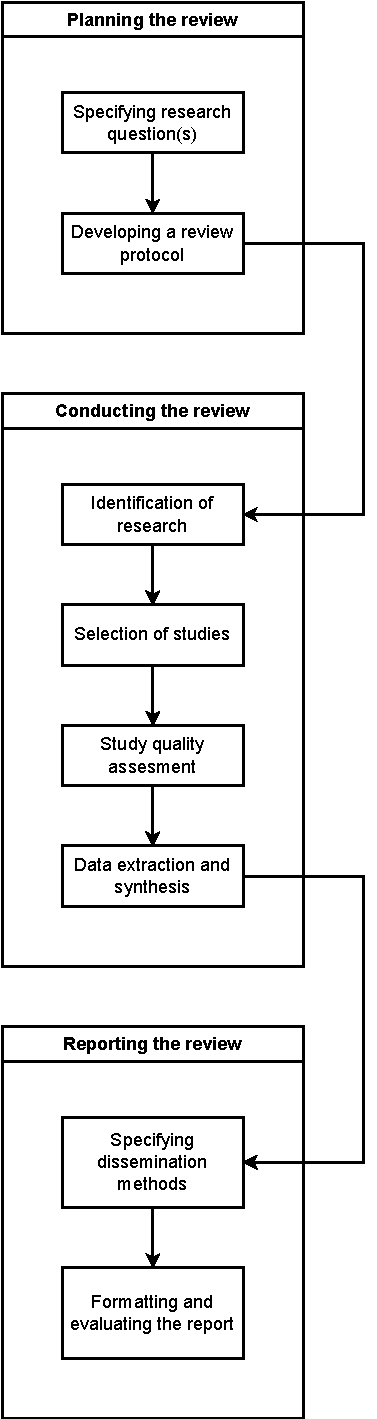
\includegraphics[scale=0.9]{figures/slr-phases.pdf}
	\caption{Three phases of a systematic literature review}
	\label{fig:slrphases}
\end{figure}

The multivocal literature review process began with the formulation of research questions and the establishment of a comprehensive search strategy and scope. The search process was conducted by employing a quasi-gold standard (QGS) approach based on the implementation by \cite{qgs}. After the completion of the search process, the inclusion and exclusion criteria were defined, and a strategy was developed for assessing the quality of the multivocal literature that met these criteria. To ensure a structured evaluation of the literature, a data extraction form was created. Finally, a strategy for analyzing the extracted data from the literature was designed.

 To ensure the reliability and validity of the research protocol, it was validated against similar systematic literature reviews in computer science, the aforementioned guidelines by \cite{kitchenham2007}, and was further refined through an iterative process. Specifically, a subset of the data was tested on (The QGS) and any identified issues or problems were recorded and addressed. The details of this process are explained and thoroughly documented in the following sections. Similarly, the same approach was followed for the data extraction process, whereby a subset of literature was tested to refine the data extraction form. The revision of the form was undertaken as necessary to guarantee the completeness and accuracy of the extracted data.

\section{Research questions}
The research questions in this study served two primary purposes. Firstly, they aimed to provide an anaylsis of the existing multivocal literature on PCLs in software engineering for the researchers interested about the field. Secondly, the questions were designed to cater a secondary audience of professional software engineering practicioners. As discussed in the \hyperref[intro]{Chapter 1}, the following research questions were addressed in this thesis:

\begin{itemize}
	\item RQ1: How many PCLs are there in software engineering?
	\item RQ2: What is the average length of a PCL in software engineering?
	\item RQ3: How often do PCLs in software engineering change?
	\item RQ4: How have PCLs in software engineering changed?
	\item RQ5: Why do PCLs in software engineering get new versions?
\end{itemize}

The multivocal literature review in this thesis begins with addressing RQ1, which aims to provide the amount of PCLs that exist in software engineering. The review takes into account attributes like versions, supersedences to a different license family, formal or otherwise and recognizability. These attributes give us different amounts to existing PCLs in software engineering. This information could be most valuable for the practicioners out of all the research questions in the thesis since it could give some sense of the scale when picking a PCL that would serve the practicioners' needs the best.

Next RQ2 seeks to find the average length of the text of a PCL in software engineering. This research question has attributes like the number of characters, sentences, distinct sections and the size of the license on a computer screen. This information could be valuable for the practicioners mentioned in the previous parapgrah for the same reasons of getting a better overview of the PCLs in software engineering. The research questions could also be beneficial for the practicioners working directly within the meta plane of PCLs in software engineering. Let us refer to the latter as researchers.

Finally RQs 3 to 5 review changes related to PCLs in software engineering. The research questions go over the average length of time between new changes to the licenses and their corresponding versions, the content of the changes and the implied and expressed reasons for making the changes. The answers to these three research questions could again be useful for the researchers. The results can be used to introduce some notable background of the current PCLs in software engineering and enabling focus to more specific areas inside this PCLs in software engineering.

\section{Search stragey}
The search process was conducted in Google Search. The selection criteria for the literature were defined after the search process and the selection process was based on inclusion and exclusion criteria. The inclusion and exclusion criteria and each step of exclusion on the literature found was documented and is available as \hyperref[appendix:a]{Appendix A}. The used criteria are presented later in this chapter.

The data extraction process was performed in a standardized and systematic manner, with the aim of obtaining all relevant information from the selected literature. The data extraction form used included information such as license name, release year, text length and inferred purpose and is available  \hyperref[table:extraction]{Table 2.1}. The extracted data was then used to answer the research questions and perform the data analysis. The results of the data analysis were then reported in a rigorous manner.
\subsection{Search method}
The search was conducted on Google Search, as mentioned earlier, to obtain a broad set of multivocal literature. This approach yielded a large number of literature that were processed to a subset of high-relevance literature using exclusion and quality criteria presented later in this chapter. Manual searching of databases with thousands of PCLs is not feasible, and it is prone to researcher bias and may overlook relevant venues from other scientific disciplines. However, a preliminary manual search was performed to reduce the number of iterations required and establish the quasi-gold standard (QGS) mentioned earlier.
\subsection{Search scope and terms}
EPLAIN WHY THIS DID NOT HAPPEN EITHER
The search terms for this study were determined through an iterative process that took into account the research questions and topic.

EXPLAIN WHY QGS SEARCH STRING COULD NOT BE DONE BUT WIKIPEDIA INSTEAD
The search string was established on a basis of a quasi-gold standard as proposed by \cite{qgs}. For establishing a QGS we employed a manually crafted search string based on the topic and research questions of this study. As we defined PCLs in software engineering as copyright licenses where the licensees are not limited and the copyright license in question is meant be used in licensing software source code in \hyperref[methods]{Chapter 2} and our research questions focus on finding measurements and reasonings to the PCLs' various attributes, we manually formulated the search string:

\section{Search process}
\section{Inclusion and exclusion criteria}
\section{Quality and evidence criteria}
\section{Data collection and data analysis}
\begin{table}[t]
	\begin{center}
		\begin{tabular}{||c c c||} 
			\hline
			\# & Field & Concern/Research question \\
			\hline
			F1 & Name & Documentation \\
			F2 & Year & RQ3, RQ4, RQ5 \\
			F3 & Length & RQ2 \\
			F4 & Inferred purpose & RQ1, RQ5 \\
			F3 & FSF approval &  Documentation\\
			F4 & OSI approval & Documentation \\
			\hline
		\end{tabular}
		\caption{Data extraction form}
		\label{table:extraction}
	\end{center}
\end{table}